\PassOptionsToPackage{unicode=true}{hyperref} % options for packages loaded elsewhere
\PassOptionsToPackage{hyphens}{url}
%
\documentclass[
  9pt,
  ignorenonframetext,
]{beamer}
\usepackage{pgfpages}
\setbeamertemplate{caption}[numbered]
\setbeamertemplate{caption label separator}{: }
\setbeamercolor{caption name}{fg=normal text.fg}
\beamertemplatenavigationsymbolsempty
% Prevent slide breaks in the middle of a paragraph:
\widowpenalties 1 10000
\raggedbottom
\setbeamertemplate{part page}{
  \centering
  \begin{beamercolorbox}[sep=16pt,center]{part title}
    \usebeamerfont{part title}\insertpart\par
  \end{beamercolorbox}
}
\setbeamertemplate{section page}{
  \centering
  \begin{beamercolorbox}[sep=12pt,center]{part title}
    \usebeamerfont{section title}\insertsection\par
  \end{beamercolorbox}
}
\setbeamertemplate{subsection page}{
  \centering
  \begin{beamercolorbox}[sep=8pt,center]{part title}
    \usebeamerfont{subsection title}\insertsubsection\par
  \end{beamercolorbox}
}
\AtBeginPart{
  \frame{\partpage}
}
\AtBeginSection{
  \ifbibliography
  \else
    \frame{\sectionpage}
  \fi
}
\AtBeginSubsection{
  \frame{\subsectionpage}
}
\usepackage{lmodern}
\usepackage{amssymb,amsmath}
\usepackage{ifxetex,ifluatex}
\ifnum 0\ifxetex 1\fi\ifluatex 1\fi=0 % if pdftex
  \usepackage[T1]{fontenc}
  \usepackage[utf8]{inputenc}
  \usepackage{textcomp} % provides euro and other symbols
\else % if luatex or xelatex
  \usepackage{unicode-math}
  \defaultfontfeatures{Scale=MatchLowercase}
  \defaultfontfeatures[\rmfamily]{Ligatures=TeX,Scale=1}
\fi
\usetheme[]{Boadilla}
\usecolortheme{seahorse}
% use upquote if available, for straight quotes in verbatim environments
\IfFileExists{upquote.sty}{\usepackage{upquote}}{}
\IfFileExists{microtype.sty}{% use microtype if available
  \usepackage[]{microtype}
  \UseMicrotypeSet[protrusion]{basicmath} % disable protrusion for tt fonts
}{}
\makeatletter
\@ifundefined{KOMAClassName}{% if non-KOMA class
  \IfFileExists{parskip.sty}{%
    \usepackage{parskip}
  }{% else
    \setlength{\parindent}{0pt}
    \setlength{\parskip}{6pt plus 2pt minus 1pt}}
}{% if KOMA class
  \KOMAoptions{parskip=half}}
\makeatother
\usepackage{xcolor}
\IfFileExists{xurl.sty}{\usepackage{xurl}}{} % add URL line breaks if available
\IfFileExists{bookmark.sty}{\usepackage{bookmark}}{\usepackage{hyperref}}
\hypersetup{
  pdftitle={Master en Big Data. Fundamentos matemáticos del análisis de datos.},
  pdfauthor={Fernando San Segundo},
  pdfborder={0 0 0},
  breaklinks=true}
\urlstyle{same}  % don't use monospace font for urls
\newif\ifbibliography
\usepackage{color}
\usepackage{fancyvrb}
\newcommand{\VerbBar}{|}
\newcommand{\VERB}{\Verb[commandchars=\\\{\}]}
\DefineVerbatimEnvironment{Highlighting}{Verbatim}{commandchars=\\\{\}}
% Add ',fontsize=\small' for more characters per line
\usepackage{framed}
\definecolor{shadecolor}{RGB}{248,248,248}
\newenvironment{Shaded}{\begin{snugshade}}{\end{snugshade}}
\newcommand{\AlertTok}[1]{\textcolor[rgb]{0.94,0.16,0.16}{#1}}
\newcommand{\AnnotationTok}[1]{\textcolor[rgb]{0.56,0.35,0.01}{\textbf{\textit{#1}}}}
\newcommand{\AttributeTok}[1]{\textcolor[rgb]{0.77,0.63,0.00}{#1}}
\newcommand{\BaseNTok}[1]{\textcolor[rgb]{0.00,0.00,0.81}{#1}}
\newcommand{\BuiltInTok}[1]{#1}
\newcommand{\CharTok}[1]{\textcolor[rgb]{0.31,0.60,0.02}{#1}}
\newcommand{\CommentTok}[1]{\textcolor[rgb]{0.56,0.35,0.01}{\textit{#1}}}
\newcommand{\CommentVarTok}[1]{\textcolor[rgb]{0.56,0.35,0.01}{\textbf{\textit{#1}}}}
\newcommand{\ConstantTok}[1]{\textcolor[rgb]{0.00,0.00,0.00}{#1}}
\newcommand{\ControlFlowTok}[1]{\textcolor[rgb]{0.13,0.29,0.53}{\textbf{#1}}}
\newcommand{\DataTypeTok}[1]{\textcolor[rgb]{0.13,0.29,0.53}{#1}}
\newcommand{\DecValTok}[1]{\textcolor[rgb]{0.00,0.00,0.81}{#1}}
\newcommand{\DocumentationTok}[1]{\textcolor[rgb]{0.56,0.35,0.01}{\textbf{\textit{#1}}}}
\newcommand{\ErrorTok}[1]{\textcolor[rgb]{0.64,0.00,0.00}{\textbf{#1}}}
\newcommand{\ExtensionTok}[1]{#1}
\newcommand{\FloatTok}[1]{\textcolor[rgb]{0.00,0.00,0.81}{#1}}
\newcommand{\FunctionTok}[1]{\textcolor[rgb]{0.00,0.00,0.00}{#1}}
\newcommand{\ImportTok}[1]{#1}
\newcommand{\InformationTok}[1]{\textcolor[rgb]{0.56,0.35,0.01}{\textbf{\textit{#1}}}}
\newcommand{\KeywordTok}[1]{\textcolor[rgb]{0.13,0.29,0.53}{\textbf{#1}}}
\newcommand{\NormalTok}[1]{#1}
\newcommand{\OperatorTok}[1]{\textcolor[rgb]{0.81,0.36,0.00}{\textbf{#1}}}
\newcommand{\OtherTok}[1]{\textcolor[rgb]{0.56,0.35,0.01}{#1}}
\newcommand{\PreprocessorTok}[1]{\textcolor[rgb]{0.56,0.35,0.01}{\textit{#1}}}
\newcommand{\RegionMarkerTok}[1]{#1}
\newcommand{\SpecialCharTok}[1]{\textcolor[rgb]{0.00,0.00,0.00}{#1}}
\newcommand{\SpecialStringTok}[1]{\textcolor[rgb]{0.31,0.60,0.02}{#1}}
\newcommand{\StringTok}[1]{\textcolor[rgb]{0.31,0.60,0.02}{#1}}
\newcommand{\VariableTok}[1]{\textcolor[rgb]{0.00,0.00,0.00}{#1}}
\newcommand{\VerbatimStringTok}[1]{\textcolor[rgb]{0.31,0.60,0.02}{#1}}
\newcommand{\WarningTok}[1]{\textcolor[rgb]{0.56,0.35,0.01}{\textbf{\textit{#1}}}}
\setlength{\emergencystretch}{3em}  % prevent overfull lines
\providecommand{\tightlist}{%
  \setlength{\itemsep}{0pt}\setlength{\parskip}{0pt}}
\setcounter{secnumdepth}{-2}

% set default figure placement to htbp
\makeatletter
\def\fps@figure{htbp}
\makeatother

% Adaptado de http://rmarkdown.rstudio.com/articles_beamer.html

\usepackage[spanish, es-tabla, es-nodecimaldot]{babel}

%\usepackage{multirow}
%\usepackage{graphicx}
%\usepackage{rotating}
%\setbeamertemplate{caption}[numbered]
%\usepackage{hyperref}
%\usepackage{caption}
%\usepackage[normalem]{ulem}
%	\mode<presentation>
%\usepackage{wasysym}
\usepackage{amsmath}
%\usepackage{array}
%\usetheme{Warsaw}
%\usecolortheme{spruce}
%\usepackage{attachfile}
%\usepackage[dvipsnames]{xcolor}
%\definecolor{DarkGreen}{HTML}{009900}



\AtBeginSection{\frame{\sectionpage}}
\AtBeginSubsection{\frame{\subsectionpage}}
\newtranslation[to=spanish]{Section}{Secci\'on}
\newtranslation[to=spanish]{Subsection}{Subsecci\'on}

\usepackage{keystroke}


% logo of my university
\titlegraphic{
\includegraphics[width=4cm]{../fig/logoICAI.png}}

\title{Master en Big Data. Fundamentos matemáticos del análisis de datos.}
\subtitle{Sesión 2: Tipos de Variables y Análisis Exploratorio}
\author{Fernando San Segundo}
\date{Curso 2019-20. Última actualización: 2019-08-30}

\begin{document}
\frame{\titlepage}

\begin{frame}
  \tableofcontents[hideallsubsections]
\end{frame}
\hypertarget{trabajando-con-ficheros-de-datos.}{%
\section{Trabajando con ficheros de
datos.}\label{trabajando-con-ficheros-de-datos.}}

\begin{frame}

\begin{center}\includegraphics[width=0.7\linewidth]{02-TiposDeVariablesEDA_files/figure-beamer/unnamed-chunk-2-1} \end{center}

\href{https://xkcd.com/1301/}{\textcolor{blue}{\underline{XKCD}}}

\end{frame}

\begin{frame}

\begin{itemize}
\tightlist
\item
  En la primera sesión hemos usado tablas de datos incorporadas en R (o
  en librerías). Pero para nuestro trabajo necesitaremos muchas veces
  importar datos procedentes de fuentes externas. Hoy aprenderemos a
  usar datos almacenados en:

  \begin{itemize}
  \tightlist
  \item
    ficheros de texto
  \item
    ficheros Excel
  \item
    ficheros de otros programas estadísticos (SAS, SPSS, etc.)
  \item
    ficheros RData propios de R Vamos a ver como leer estos ficheros
    para usar los datos en R y también veremos como guardar datos desde
    R en algunos de esos formatos.
  \end{itemize}
\end{itemize}

\({ }\)

\begin{itemize}
\tightlist
\item
  En otro momento del curso hablaremos de formas alternativas de acceder
  a datos no almacenados en ficheros (APIs, bases de datos tipo SQL, Web
  Scrapping, etc.)
\end{itemize}

\end{frame}

\begin{frame}{Ficheros de tipo csv}
\protect\hypertarget{ficheros-de-tipo-csv}{}

\begin{itemize}
\item
  El nombre csv proviene de \emph{comma separated values}, valores
  separados por comas, aunque vamosa ver enseguida que no hay que
  tomarse el nombre al pie de la letra.
\item
  Un fichero csv es un fichero de \emph{texto plano} que contiene una
  tabla de datos. Cada fila del fichero contiene una fila de la tabla y,
  dentro de esa fila, los elementos correspondientes a cada columna de
  la tabla se separan mediante comas o espacios o tabuladores, etc. La
  siguiente figura muestra uno de esos ficheros abierto en el \emph{Bloc
  de Notas} de Windows y la tabla correspondiente (se muestran las
  primeras filas).

  \begin{center}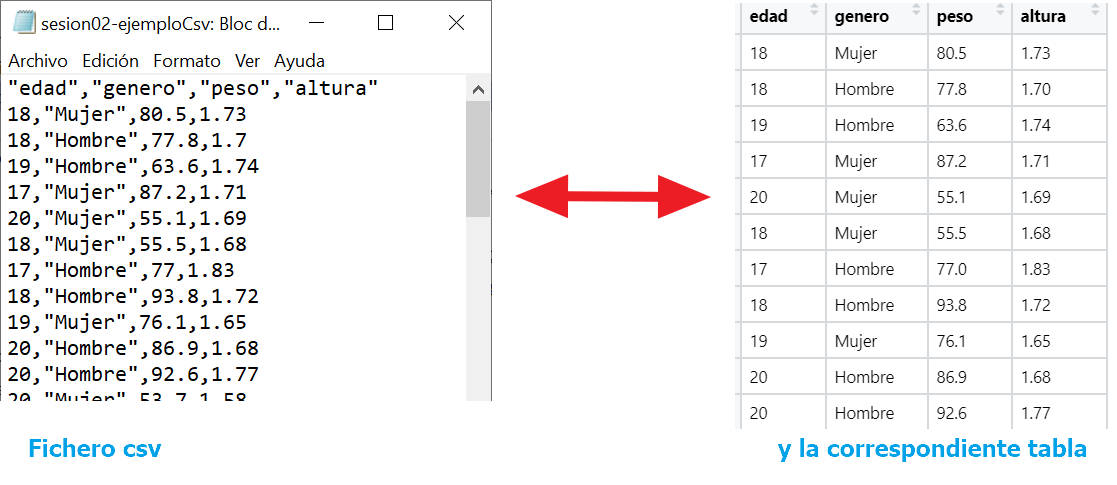
\includegraphics[width=0.8\linewidth]{../fig/02-fig01-FicherosCsv} \end{center}
\end{itemize}

\end{frame}

\begin{frame}[fragile]{Ficheros csv con R.}
\protect\hypertarget{ficheros-csv-con-r.}{}

\begin{itemize}
\item
  Vamos a empezar descargando uno de estos ficheros, llamado
  \texttt{movies.csv} que contiene datos sobre las
  \href{https://gist.githubusercontent.com/tiangechen/b68782efa49a16edaf07dc2cdaa855ea/raw/0c794a9717f18b094eabab2cd6a6b9a226903577/movies.csv}{\textcolor{blue}{\underline{películas más taquilleras  entre 2007 y 2011}}}.
\item
  Recuerda que debes indicarle a RStudio el \emph{Directorio de Trabajo}
  y que el fichero descargado debe estar almacenado en la subcarpeta
  \emph{datos} de ese directorio de trabajo.
\item
  Empieza abriendo ese fichero en un editor de texto (tipo \emph{Bloc de
  Notas}) para hacer una exploración preliminar.
\item
  Para abrir ese fichero con R vamos a empezar usando: \small

\begin{Shaded}
\begin{Highlighting}[]
\NormalTok{movies =}\StringTok{ }\KeywordTok{read.csv}\NormalTok{(}\DataTypeTok{file =} \StringTok{"../datos/movies.csv"}\NormalTok{, }\DataTypeTok{header =} \OtherTok{TRUE}\NormalTok{)}
\end{Highlighting}
\end{Shaded}
\end{itemize}

\normalsize

\begin{itemize}
\item
  El resultado de este comando es un data.frame de R. Las opciones de la
  función son:

  \begin{itemize}
  \tightlist
  \item
    \emph{file}: el nombre y directorio del fichero relativo (a la
    carpeta de trabajo).
  \item
    \emph{header}: que puede ser TRUE o FALSE, para indicar si la
    primera fila del csv contiene los nombres de las variables.
  \end{itemize}

  Veremos más adelante otras opciones importantes de esta función y
  funciones similares.
\end{itemize}

\end{frame}

\begin{frame}[fragile]

\begin{block}{Repaso de operaciones con data.frames.}

\begin{itemize}
\item
  Recuerda que puedes seleccionar por filas con instrucciones como:
  \tiny

\begin{Shaded}
\begin{Highlighting}[]
\NormalTok{movies[}\DecValTok{7}\NormalTok{, ]}
\end{Highlighting}
\end{Shaded}

\begin{verbatim}
##     Film     Genre Lead.Studio Audience.score..
## 7 WALL-E Animation      Disney               89
##   Profitability Rotten.Tomatoes.. Worldwide.Gross Year
## 7      2.896019                96        $521.28  2008
\end{verbatim}
\end{itemize}

\normalsize \({ }\)

\begin{itemize}
\item
  Y por columnas de forma similar o también por nombre de variable
  usando \texttt{\$}: \scriptsize

\begin{Shaded}
\begin{Highlighting}[]
\KeywordTok{tail}\NormalTok{(movies}\OperatorTok{$}\NormalTok{Year, }\DecValTok{20}\NormalTok{) }\CommentTok{# se muestran las 20 últimas}
\end{Highlighting}
\end{Shaded}

\begin{verbatim}
##  [1] 2011 2009 2010 2008 2009 2007 2010 2011 2011 2009 2008
## [12] 2008 2007 2010 2011 2007 2009 2011 2008 2009
\end{verbatim}
\end{itemize}

\normalsize \({ }\)

\begin{itemize}
\item
  Recuerda asimismo que puedes seleccionar por condiciones. Por ejemplo
  para ver el género de las películas de 2010 con:

\begin{Shaded}
\begin{Highlighting}[]
\NormalTok{movies}\OperatorTok{$}\NormalTok{Genre[movies}\OperatorTok{$}\NormalTok{Year }\OperatorTok{==}\StringTok{ }\DecValTok{2010}\NormalTok{]}
\end{Highlighting}
\end{Shaded}

  También sabemos usar \texttt{dplyr} para seleccionar: \scriptsize

\begin{Shaded}
\begin{Highlighting}[]
\NormalTok{movies }\OperatorTok\StringTok{ }
\StringTok{  }\KeywordTok{filter}\NormalTok{(Year }\OperatorTok{==}\StringTok{ }\DecValTok{2010}\NormalTok{) }\OperatorTok\StringTok{ }
\StringTok{  }\KeywordTok{select}\NormalTok{(Genre) }\OperatorTok\StringTok{ }
\StringTok{  }\NormalTok{.[}\DecValTok{1}\OperatorTok{:}\DecValTok{20}\NormalTok{, ]     }\CommentTok{# ¿Qué hace esta última operación?}
\end{Highlighting}
\end{Shaded}

\begin{verbatim}
##  [1] Comedy    Comedy    Comedy    Comedy    Comedy   
##  [6] Animation Comedy    Comedy    Comedy    Drama    
## [11] Comedy    Comedy    Comedy    Comedy    Comedy   
## [16] Action    Comedy    Comedy    Comedy    Drama    
## 10 Levels: Action Animation Comdy comedy Comedy ... Romence
\end{verbatim}
\end{itemize}

\normalsize \({ }\)

\begin{itemize}
\tightlist
\item
  \textbf{Ejercicio:} ¿Cuál es la película más taquillera? ¿Cuál es el
  género de esa película?
\end{itemize}

\end{block}

\end{frame}

\begin{frame}[fragile]{Usando readr para leer y escribir ficheros csv.}
\protect\hypertarget{usando-readr-para-leer-y-escribir-ficheros-csv.}{}

\begin{itemize}
\item
  La librería \texttt{readr}, que forma parte del tidyverse, incluye la
  función \texttt{read\_csv}, que es muy fácil de usar y muy rápida para
  ficheros grandes. Explora esta tabla como hemos hecho con la primera
  versión.\\
  \small

\begin{Shaded}
\begin{Highlighting}[]
\KeywordTok{library}\NormalTok{(tidyverse)}
\NormalTok{movies2 =}\StringTok{ }\KeywordTok{read_csv}\NormalTok{(}\StringTok{"../datos/movies.csv"}\NormalTok{)}
\end{Highlighting}
\end{Shaded}
\end{itemize}

\normalsize

\begin{itemize}
\item
  También puedes usar readr para crear ficheros csv a partir de una
  tabla (por ejemplo un data.frame) en R. El siguiente código genera
  primero una tabla con tres variables A, B y C y a continuación guarda
  esa tabla a un fichero csv. Asegúrate de abrir el fichero resultante
  en un editor de texto para ver el resultado. \small

\begin{Shaded}
\begin{Highlighting}[]
\NormalTok{datos =}\StringTok{ }
\StringTok{  }\KeywordTok{data.frame}\NormalTok{(}\DataTypeTok{A =} \KeywordTok{sample}\NormalTok{(}\DecValTok{1}\OperatorTok{:}\DecValTok{100}\NormalTok{, }\DecValTok{10}\NormalTok{), }\DataTypeTok{B =} \KeywordTok{sample}\NormalTok{(LETTERS, }\DecValTok{10}\NormalTok{), }\DataTypeTok{C =} \KeywordTok{rnorm}\NormalTok{(}\DecValTok{10}\NormalTok{))}
\KeywordTok{head}\NormalTok{(datos, }\DecValTok{2}\NormalTok{)}
\KeywordTok{write_csv}\NormalTok{(datos, }\DataTypeTok{path =} \StringTok{"../datos/sesion02-guardarCsv.csv"}\NormalTok{)}
\end{Highlighting}
\end{Shaded}

\begin{verbatim}
##    A B          C
## 1 25 N -0.1114757
## 2 42 Q -2.3553230
\end{verbatim}
\end{itemize}

\normalsize

\begin{itemize}
\tightlist
\item
  Las funciones \texttt{write.table} y \texttt{write.csv} de R funcionan
  de manera parecida. Veremos algún ejemplo de uso más adelante.
\end{itemize}

\end{frame}

\begin{frame}[fragile]{Ficheros Excel}
\protect\hypertarget{ficheros-excel}{}

\begin{itemize}
\item
  Las hojas de cálculo y en particular Excel son una herramienta muy
  utilizada. Por eso no es infrecuente encontrarse con ficheros de datos
  que se han almacenado en alguno de los formatos propios de diferentes
  versiones de Excel.
\item
  Descarga para usar como ejemplo
  \href{http://users.stat.ufl.edu/~winner/data/train_acc_2010.xls}{este
  fichero} en formato xls, que contiene datos sobre accidentes
  ferroviarios ocurridos en 2010 en los Estados Unidos. Puedes encontrar
  más detalles sobre el fichero en
  \href{http://users.stat.ufl.edu/~winner/data/train_acc_2010.txt}{\textcolor{blue}{\underline{este documento auxiliar}}}.
\item
  Para leer esos datos vamos a usar la librería \texttt{readxl} de esta
  forma

\begin{Shaded}
\begin{Highlighting}[]
\KeywordTok{library}\NormalTok{(readxl)}
\NormalTok{accidentes =}\StringTok{ }\KeywordTok{read_excel}\NormalTok{(}\StringTok{"../datos/train_acc_2010.xls"}\NormalTok{)}
\end{Highlighting}
\end{Shaded}
\item
  \textbf{Ejercicio:} exporta esta tabla de R a un fichero en formato
  csv llamado \texttt{accidentes.csv}.
\end{itemize}

\end{frame}

\begin{frame}[fragile]{Ficheros de otros programas estadísticos.}
\protect\hypertarget{ficheros-de-otros-programas-estadisticos.}{}

\begin{itemize}
\item
  Aunque existen muchos otros programas estadísticos, aquí solo vamos a
  ver como se usa la libraría \texttt{haven} del tidyverse para importar
  en R ficheros de datos de SPSS, Stata y SAS. Si necesitas importar
  datos almacenados en un formato propio de otro programa lo mejor es
  buscar en Internet algo como \emph{import from \ldots{} to R}.
  Recuerda empezar cargando la librería.

\begin{Shaded}
\begin{Highlighting}[]
\KeywordTok{library}\NormalTok{(haven)}
\end{Highlighting}
\end{Shaded}
\end{itemize}

\begin{block}{Fichero SAV de SPSS}

\begin{itemize}
\item
  Descarga el fichero \texttt{CH10\_Planet\_distances\_and\_y.SAV} a la
  carpeta datos desde
  \href{http://media.pearsoncmg.com/aw/aw_deveaux_stats_2/activstats/spss/CH10_Planet_distances_and_y.SAV}{\textcolor{blue}{\underline{este enlace}}}
  y ábrelo con: \scriptsize

\begin{Shaded}
\begin{Highlighting}[]
\KeywordTok{library}\NormalTok{(haven)}
\NormalTok{planetas =}\StringTok{ }\KeywordTok{read_spss}\NormalTok{(}\StringTok{"../datos/CH10_Planet_distances_and_y.SAV"}\NormalTok{)}
\KeywordTok{head}\NormalTok{(planetas, }\DecValTok{3}\NormalTok{) }\CommentTok{# Veamos las tres primeras filas.}
\end{Highlighting}
\end{Shaded}

\begin{verbatim}
## # A tibble: 3 x 4
##   Planet  PositionNumber Distancefromsunmillionmiles Lengthofyearearthyears
##   <chr>            <dbl>                       <dbl>                  <dbl>
## 1 Mercury              1                          36                   0.24
## 2 Venus                2                          67                   0.61
## 3 Earth                3                          93                   1
\end{verbatim}
\end{itemize}

\normalsize

\end{block}

\end{frame}

\begin{frame}[fragile]

\begin{block}{Ficheros sas7bdat de SAS y dta de Stata}

\begin{itemize}
\item
  Usa
  \href{http://www.principlesofeconometrics.com/sas/transport.sas7bdat}{\textcolor{blue}{\underline{este enlace}}}
  para descargar el fichero \texttt{transport.sas7bdat} a la carpeta
  datos y ábrelo con: \scriptsize

\begin{Shaded}
\begin{Highlighting}[]
\NormalTok{transport =}\StringTok{ }\KeywordTok{read_sas}\NormalTok{(}\StringTok{"../datos/transport.sas7bdat"}\NormalTok{)}
\KeywordTok{head}\NormalTok{(transport, }\DecValTok{3}\NormalTok{) }
\end{Highlighting}
\end{Shaded}

\begin{verbatim}
## # A tibble: 3 x 4
##   AUTOTIME BUSTIME DTIME  AUTO
##      <dbl>   <dbl> <dbl> <dbl>
## 1    52.9     4.40 -48.5     0
## 2     4.10   28.5   24.4     0
## 3     4.10   86.9   82.8     1
\end{verbatim}
\end{itemize}

\normalsize

\({ }\)

\begin{itemize}
\item
  Procede de forma análoga con
  \href{http://www.stata-press.com/data/r8/auto2.dta}{\textcolor{blue}{\underline{este fichero}}}
  llamado \texttt{auto2.dta} en formato de Stata\\
  \tiny

\begin{Shaded}
\begin{Highlighting}[]
\NormalTok{auto2 =}\StringTok{ }\KeywordTok{read_dta}\NormalTok{(}\StringTok{"../datos/auto2.dta"}\NormalTok{)}
\KeywordTok{head}\NormalTok{(auto2, }\DecValTok{3}\NormalTok{) }
\end{Highlighting}
\end{Shaded}

\begin{verbatim}
## # A tibble: 3 x 13
##   make        price   mpg rep78 headroom trunk weight length  turn displacement gear_ratio      foreign weightsq
##   <chr>       <dbl> <dbl> <dbl>    <dbl> <dbl>  <dbl>  <dbl> <dbl>        <dbl>      <dbl>    <dbl+lbl>    <dbl>
## 1 AMC Concord  4099    22     3      2.5    11   2930    186    40          121       3.58 0 [Domestic]  8584900
## 2 AMC Pacer    4749    17     3      3      11   3350    173    40          258       2.53 0 [Domestic] 11222500
## 3 AMC Spirit   3799    22    NA      3      12   2640    168    35          121       3.08 0 [Domestic]  6969600
\end{verbatim}
\end{itemize}

\normalsize

\begin{itemize}
\tightlist
\item
  Guarda ambos ficheros en formato csv en la carpeta datos, los usaremos
  después como ejemplos.
\end{itemize}

\end{block}

\begin{block}{}

\begin{itemize}
\tightlist
\item
  Como ves todos los casos se gestionan de forma muy parecida. En
  ejemplos posteriores veremos otras situaciones; como tratar por
  ejemplo con ficheros comprimidos tipo zip.
\end{itemize}

\end{block}

\end{frame}

\begin{frame}[fragile]{Ficheros RData.}
\protect\hypertarget{ficheros-rdata.}{}

\begin{itemize}
\item
  R también posee su propio formato de almacenamiento de objetos, usando
  ficheros tipo RData. Estos ficheros pueden contener varias tablas de
  datos, variables y otros objetos de R. Por ejemplo podemos guardar la
  tabla de accidentes ferroviarios y la de planetas que hemos usado
  antes mediante: \small

\begin{Shaded}
\begin{Highlighting}[]
\KeywordTok{save}\NormalTok{(}\StringTok{"accidentes"}\NormalTok{, }\StringTok{"planetas"}\NormalTok{, }\DataTypeTok{file =} \StringTok{"../datos/accidentes_planetas.RData"}\NormalTok{)}
\end{Highlighting}
\end{Shaded}
\end{itemize}

\normalsize

\begin{itemize}
\item
  Fíjate en que hemos añadido la extensión RData manualmente, porque R
  no lo hace por defecto. Ahora vamos a eliminar por ejemplo la tabla
  planetas con:

\begin{Shaded}
\begin{Highlighting}[]
\KeywordTok{rm}\NormalTok{(planetas)}
\end{Highlighting}
\end{Shaded}

  Comprueba mirando el panel de entorno que en efecto la tabla ha
  desaparecido y si intentas usarla R lanzará un mensaje de error. Y
  ahora para recuperar esos datos usa: \scriptsize

\begin{Shaded}
\begin{Highlighting}[]
\KeywordTok{load}\NormalTok{(}\DataTypeTok{file =} \StringTok{"../datos/accidentes_planetas.RData"}\NormalTok{)}
\KeywordTok{head}\NormalTok{(planetas, }\DecValTok{3}\NormalTok{)}
\end{Highlighting}
\end{Shaded}

\begin{verbatim}
## # A tibble: 3 x 4
##   Planet  PositionNumber Distancefromsunmillionmiles Lengthofyearearthyears
##   <chr>            <dbl>                       <dbl>                  <dbl>
## 1 Mercury              1                          36                   0.24
## 2 Venus                2                          67                   0.61
## 3 Earth                3                          93                   1
\end{verbatim}
\end{itemize}

\normalsize

\end{frame}

\hypertarget{tipos-de-variables.}{%
\section{Tipos de Variables.}\label{tipos-de-variables.}}

\begin{frame}[fragile]

\begin{itemize}
\item
  Los tablas de datos que hemos leído en los ficheros de la sección
  previa contienen variables de distintos tipos: números enteros, con
  decimales, fechas, variables binarias de tipo sí/no, hombre/mujer,
  ubicaciones, etc. Existen muchos tipos de datos distintos, que
  permiten distintas operaciones con ellos.
\item
  En las próximas secciones vamos a conocer las categorías básicas de
  datos y las formas más adecuadas de describirlos. Como ejemplos
  iniciales vamos a usar la tabla \texttt{mpg} conyenida en la librería
  \texttt{tidyverse} y también una tabla con datos relativos a un
  estudio sobre enfermades coronarias llevado a cabo a Framingham (UK).
  Puedes descargar el fichero csv desde
  \href{https://raw.githubusercontent.com/fernandosansegundo/MBDFME/master/datos/framingham.csv}{\textcolor{blue}{\underline{este enlace}}}
  y leer más detalles sobre el estudio
  \href{https://biolincc.nhlbi.nih.gov/media/teachingstudies/FHS_Teaching_Longitudinal_Data_Documentation.pdf?link_time=2019-08-26_14:42:24.487245}{\textcolor{blue}{\underline{aquí}}.}.
\item
  \textbf{Ejercicio:} lee el fichero a una tabla de R llamada fhs (de
  Framingham Heart Study). Explora esa tabla con las funciones
  \texttt{str} y \texttt{glimpse}. Piensa en qué tipo de información
  contiene cada variable de la tabla. Lee también la documentación sobre
  \texttt{mpg} en
  \href{https://ggplot2.tidyverse.org/reference/mpg.html}{\textcolor{blue}{\underline{este enlace}}}.
\end{itemize}

\begin{center}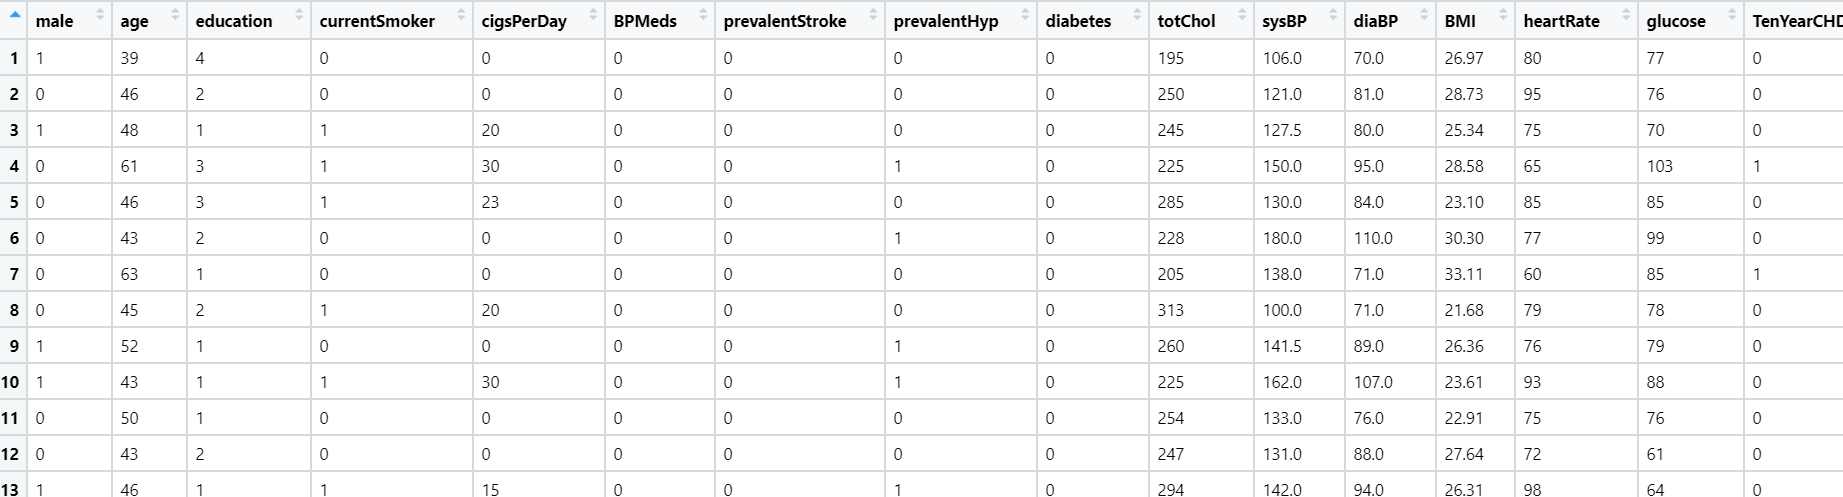
\includegraphics[width=0.8\linewidth]{../fig/02-fig02-fhs} \end{center}

\end{frame}

\begin{frame}{Clasificación inicial.}
\protect\hypertarget{clasificacion-inicial.}{}

\begin{itemize}
\item
  Los datos que han ido apareciendo en nuestros ejemplos se pueden
  clasificar en:

  \begin{itemize}
  \tightlist
  \item
    \textbf{Datos Cuantitativos (Numéricos):} que a su vez se dividen en
    \textbf{discretos} y \textbf{continuos}.\\
  \item
    \textbf{Datos Cualitativos (Factores)}: que pueden ser o no
    ordenados.
  \end{itemize}
\item
  Esta es la clasificación tradicional en muchos cursos de introducción
  a la Estadística y enseguida vamos a ver ejemplos para entender la
  diferencia entre estos tipos de datos, Pero queremos subrayar que
  existen muchos tipos de datos estructurados de uso frecuente que
  superan esta clasificación tradicional (fechas, imágenes, ficheros de
  audio o vídeo).
\item
  Primero vamos a aprender a analizar variables individuales, por
  separado, antes de preguntarnos por las relaciones entre ellas.
\end{itemize}

\end{frame}

\begin{frame}[fragile]

\begin{itemize}
\item
  Una \emph{variable cuantitativa} (discreta o continua) es una variable
  que toma valores numéricos que \emph{además} se han medido en alguna
  escala que permite interpretarlos y hacer operaciones aritméticas
  (sumas, productos, etc) con ellos.
\item
  Una variable cuantitativa es \emph{discreta} si se mide en una escala
  de unidades enteras (paso a paso, los valores se miden
  \emph{contando}). Y la variable \emph{continua} si la escala de medida
  se puede dividir arbitrariamente (se usan valores decimales). Pero
  como veremos en ejemplos, la división discreto/continuo también es
  sutil y se refiere en realidad a la forma en la que \emph{usamos} la
  variable.
\end{itemize}

\begin{center}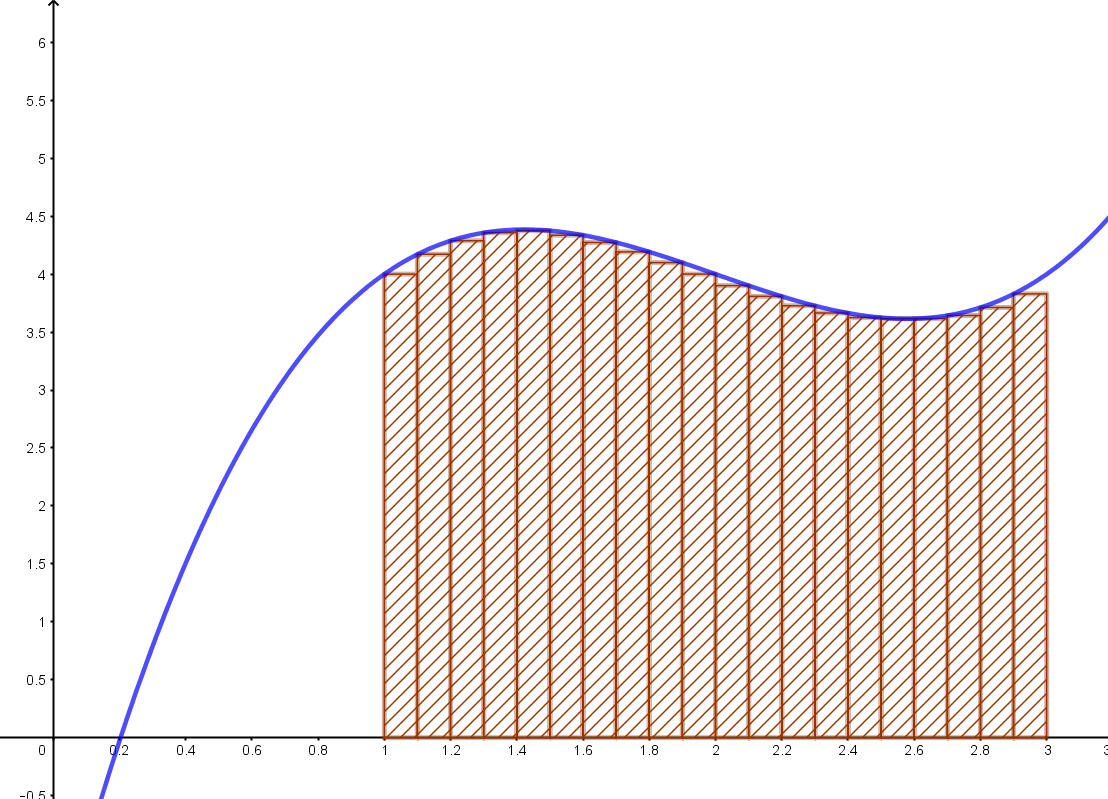
\includegraphics[width=0.2\linewidth]{../fig/02-fig03-DiscretoContinuo} \end{center}

\begin{itemize}
\item
  Podría pensarse entonces que las variables cuantitativas son las
  variables numéricas y las cualitativas las no numéricas. La diferencia
  es, en realidad, un poco más sutil. Una variable es \emph{cualitativa
  (nominal)} o un \emph{factor (no ordenado)} cuando \emph{solo} se
  utiliza para establecer categorías, para \emph{clasificar}. Podemos
  \emph{representar} los valores de una de estas variables con números,
  pero el valor numérico concreto es arbitrario, es una \emph{etiqueta}.
\item
  \textbf{Ejercicio:} Examina las variables \texttt{cty}, \texttt{disp},
  \texttt{class} y \texttt{cyl} de la tabla \texttt{mpg}. ¿De qué tipo
  crees que es cada variable?
\end{itemize}

\end{frame}

\hypertarget{variables-cuantitativas-discretas.}{%
\section{Variables cuantitativas
discretas.}\label{variables-cuantitativas-discretas.}}

\begin{frame}[fragile]{Tablas de frecuencia absolutas y relativas.}
\protect\hypertarget{tablas-de-frecuencia-absolutas-y-relativas.}{}

\begin{itemize}
\item
  La variable \texttt{cty} de \texttt{mpg} el número de millas por galón
  que el coche recorre en ciclo urbano. Fíjate en que los valores son un
  número entero de millas. En principio no hay nada que impida dar esos
  valores con decimales. Pero no es eso lo que se \emph{ha decidido}
  hacer aquí, sino que se trata como una variable discreta.
\item
  El primer paso con una variable discreta como esta es obtener una
  tabla de frecuencias (absolutas), que nos dirá qué valores toma la
  variable y cuántas veces toma cada valor. Usando \texttt{table} \small

\begin{Shaded}
\begin{Highlighting}[]
\KeywordTok{table}\NormalTok{(mpg}\OperatorTok{$}\NormalTok{cty)}
\end{Highlighting}
\end{Shaded}

\begin{verbatim}

 9 11 12 13 14 15 16 17 18 19 20 21 22 23 24 25 26 28 29 33 35 
 5 20  8 21 19 24 19 16 26 20 11 23  4  3  5  2  3  2  1  1  1 
\end{verbatim}
\end{itemize}

\normalsize

\begin{itemize}
\item
  También se puede usar la función \texttt{count} de dplyr así (se omite
  el resultado):

\begin{Shaded}
\begin{Highlighting}[]
\NormalTok{mpg }\OperatorTok
\StringTok{  }\KeywordTok{count}\NormalTok{(cty)}
\end{Highlighting}
\end{Shaded}
\end{itemize}

\end{frame}

\begin{frame}[fragile]{Tabla de frecuencias relativas.}
\protect\hypertarget{tabla-de-frecuencias-relativas.}{}

\begin{itemize}
\item
  A menudo, y especialmente cuando se usan para comparaciones, nos
  interesan más saber la fracción del total que corresponde a cada uno
  de los valores de una variable discreta. Cuando esa fracciones se
  expresan como \emph{tanto por uno} obtenemos las frecuencias
  relativas, que es fácil convertir en porcentajes.
\item
  Para obtener una tabla de frecuencias relativas usando R básico
  hacemos (hemos usado la función \texttt{signif} para controlar el
  número de cifras significativas y mejorar la presentación): \small

\begin{Shaded}
\begin{Highlighting}[]
\KeywordTok{signif}\NormalTok{(}\KeywordTok{prop.table}\NormalTok{(}\KeywordTok{table}\NormalTok{(mpg}\OperatorTok{$}\NormalTok{cty)), }\DecValTok{2}\NormalTok{)}
\end{Highlighting}
\end{Shaded}

\begin{verbatim}
## 
##      9     11     12     13     14     15     16     17     18     19 
## 0.0210 0.0850 0.0340 0.0900 0.0810 0.1000 0.0810 0.0680 0.1100 0.0850 
##     20     21     22     23     24     25     26     28     29     33 
## 0.0470 0.0980 0.0170 0.0130 0.0210 0.0085 0.0130 0.0085 0.0043 0.0043 
##     35 
## 0.0043
\end{verbatim}
\end{itemize}

\normalsize

\begin{itemize}
\item
  También se puede usar \texttt{dplyr} aunque en este caso la solución
  es más complicada que el R básico. \small

\begin{Shaded}
\begin{Highlighting}[]
\NormalTok{    mpg }\OperatorTok\StringTok{ }
\StringTok{      }\KeywordTok{count}\NormalTok{(cty) }\OperatorTok
\StringTok{        }\KeywordTok{mutate}\NormalTok{(cty, }\DataTypeTok{freq =}\NormalTok{ n }\OperatorTok{/}\StringTok{ }\KeywordTok{sum}\NormalTok{(n), }\DataTypeTok{n=}\OtherTok{NULL}\NormalTok{) }\CommentTok{# NULL aquí es como un select}
\end{Highlighting}
\end{Shaded}
\end{itemize}

\normalsize

\end{frame}

\begin{frame}[fragile]

\begin{block}{Propiedades de las frecuencias relativas.}

\begin{itemize}
\item
  Las frecuencias relativas suman siempre 1,

\begin{Shaded}
\begin{Highlighting}[]
\KeywordTok{sum}\NormalTok{(}\KeywordTok{prop.table}\NormalTok{(}\KeywordTok{table}\NormalTok{(mpg}\OperatorTok{$}\NormalTok{cty)))}
\end{Highlighting}
\end{Shaded}

\begin{verbatim}
## [1] 1
\end{verbatim}
\item
  Además las frecuencias relativas están relacionadas con la idea de
  \emph{probabilidad emprírica}. Es decir, si elegimos aleatoriamente un
  valor de la variable \texttt{cty} y repetimos esa elección muchas
  veces, la probabilidad de cada uno de los distintos valores es la
  frecuencia relativa que hemos calculado.
\end{itemize}

\end{block}

\begin{block}{Frecuencias acumuladas.}

\begin{itemize}
\item
  Las \emph{frecuencias acumuladas} se usan con variables discretas para
  responder a la pregunta \emph{``¿cuántos valores hay que sean menores
  o guales que \ldots{}?''} En R se obtienen con:

\begin{Shaded}
\begin{Highlighting}[]
\KeywordTok{cumsum}\NormalTok{(}\KeywordTok{table}\NormalTok{(mpg}\OperatorTok{$}\NormalTok{cty))}
\end{Highlighting}
\end{Shaded}

\begin{verbatim}
##   9  11  12  13  14  15  16  17  18  19  20  21  22  23  24 
##   5  25  33  54  73  97 116 132 158 178 189 212 216 219 224 
##  25  26  28  29  33  35 
## 226 229 231 232 233 234
\end{verbatim}

  que nos dice, por ejemplo, que en la tabla hay 116 valores menores o
  iguales que 16.
\end{itemize}

\end{block}

\end{frame}

\hypertarget{variables-cuantitativas-continuas}{%
\section{Variables cuantitativas
continuas,}\label{variables-cuantitativas-continuas}}

\begin{frame}[fragile]{Discreto vs continuo.}
\protect\hypertarget{discreto-vs-continuo.}{}

\begin{itemize}
\item
  Las tablas de frecuencias por valores no son útiles cuando hay muchos
  valores distintos. La tabla de frecuencias de \texttt{cty} ya era un
  poco excesiva. Pero si tratamos de calcular una tabla de frecuencia
  para la variable \texttt{age} de la tabla \texttt{fhs}

\begin{Shaded}
\begin{Highlighting}[]
\KeywordTok{table}\NormalTok{(fhs}\OperatorTok{$}\NormalTok{totChol)}
\end{Highlighting}
\end{Shaded}

  puedes comprobar que la tabla que se obtiene no es una representación
  útil de la información.
\item
  En muchos ejemplos como este las diferencias entre valores
  consecutivos no son relevantes. Las preguntas relevantes pasan a ser
  las que se refieren a intervalos de valores. Para agrupar los valores
  en intervalos en R podemos usar la función \texttt{cut}. \scriptsize

\begin{Shaded}
\begin{Highlighting}[]
\NormalTok{cholLevels =}\StringTok{ }\KeywordTok{cut}\NormalTok{(fhs}\OperatorTok{$}\NormalTok{totChol, }\DataTypeTok{breaks =} \DecValTok{10}\NormalTok{)}
\KeywordTok{head}\NormalTok{(cholLevels)}
\end{Highlighting}
\end{Shaded}

\begin{verbatim}
## [1] (166,225] (225,284] (225,284] (225,284] (284,343]
## [6] (225,284]
## 10 Levels: (106,166] (166,225] (225,284] ... (637,697]
\end{verbatim}
\end{itemize}

\normalsize

\begin{itemize}
\item
  La respuesta de R nos indica que ha dividido el \emph{recorrido} de la
  variable (de mínimo a máximo) en 10 intervalos semiabiertos de igual
  longitud. El primero incluye los valores entre 106 y 166, hasta el
  último que incluye los valores de 637 a 697.
\item
  La variable \texttt{cholLevels} que hemos fabricado es un \emph{factor
  ordenado}, Veremos más ejemplos cuando aprendamos más sobre factores.
\end{itemize}

\end{frame}

\begin{frame}

\begin{itemize}
\item
  Con las variables puramente continuas no suele haber demasiado dudas a
  la hora de reconocerlas. Pero con las variables discretas el problema
  puede ser más complicado, porque depende esencialmente del número de
  valores distintos que tome la variable. Al final, en muchos casos,
  tratar a una variable como discreta o continua es decisión de quien
  realiza el análisis.
\item
  Si una variable discreta solo toma cinco o menos valores en general es
  beneficioso pensar en ella como un \emph{factor ordenado}, que
  discutiremos más adelante.
\end{itemize}

\end{frame}

\begin{frame}[fragile]{Histogramas con R básico}
\protect\hypertarget{histogramas-con-r-basico}{}

\begin{itemize}
\item
  Una forma común de representar gráficamente la tabla de frecuencias
  una variable discreta que tome más de cinco valores distintos es
  mediante un \emph{histograma}, que es un diagrama de barras. Con R
  básico:

\begin{Shaded}
\begin{Highlighting}[]
\NormalTok{cortes =}\StringTok{ }\KeywordTok{seq}\NormalTok{(}\KeywordTok{min}\NormalTok{(mpg}\OperatorTok{$}\NormalTok{cty), }\KeywordTok{max}\NormalTok{(mpg}\OperatorTok{$}\NormalTok{cty), }\DataTypeTok{length.out =} \DecValTok{11}\NormalTok{)}
\KeywordTok{hist}\NormalTok{(mpg}\OperatorTok{$}\NormalTok{cty, }\DataTypeTok{breaks =}\NormalTok{ cortes, }\DataTypeTok{col=}\StringTok{"orange"}\NormalTok{, }\DataTypeTok{main=}\StringTok{""}\NormalTok{)}
\end{Highlighting}
\end{Shaded}

  \begin{center}\includegraphics[width=0.4\linewidth]{02-TiposDeVariablesEDA_files/figure-beamer/unnamed-chunk-29-1} \end{center}
\item
  Fíjate en que el eje horizontal contiene los valores de la variable
  mientras que el eje vertical muestra las frecuencias. Hemos usado la
  opción \texttt{breaks} combinada con \texttt{seq} para elegir los
  puntos de corte entre intervalos.
\item
  \textbf{Ejercicio.} Ejecuta \texttt{hist(mpg\$cyl)}. ¿Por qué ocurre
  esto?
\end{itemize}

\end{frame}

\begin{frame}[fragile]{Histogramas con ggplot. Número de intervalos.}
\protect\hypertarget{histogramas-con-ggplot.-numero-de-intervalos.}{}

\begin{itemize}
\item
  O usando ggplot y los mismos puntos de corte:

\begin{Shaded}
\begin{Highlighting}[]
\KeywordTok{ggplot}\NormalTok{(}\DataTypeTok{data =}\NormalTok{ mpg) }\OperatorTok{+}\StringTok{ }
\StringTok{  }\KeywordTok{geom_histogram}\NormalTok{(}\DataTypeTok{mapping =} \KeywordTok{aes}\NormalTok{(cty), }\DataTypeTok{breaks =}\NormalTok{ cortes , }\DataTypeTok{fill =} \StringTok{"orange"}\NormalTok{, }\DataTypeTok{color=}\StringTok{"black"}\NormalTok{)}
\end{Highlighting}
\end{Shaded}

  \begin{center}\includegraphics[width=0.4\linewidth]{02-TiposDeVariablesEDA_files/figure-beamer/unnamed-chunk-30-1} \end{center}
\item
  ¿Cuántos intervalos se deben usar en la construcción de un histograma?
  No hay una regla fija. Aunque R y el resto de programas utilizan
  diversos algoritmos para determinar ese número, lo cierto es que la
  respuesta depende mucho de los datos concretos con los que trabajamos.
  Por eso normalmente es necesario experimentar un poco con diversos
  valores. En cualquier caso es \emph{muy desaconsejable} utilizar menos
  de cinco intervalos (o más que \(\sqrt{n}\), siendo \(n\) el número de
  datos).
\end{itemize}

\end{frame}

\begin{frame}[fragile]{Curvas de densidad.}
\protect\hypertarget{curvas-de-densidad.}{}

\begin{itemize}
\item
  La \emph{curva de densidad} es un tipo de diagrama alternativo al
  histograma. Por ejemplo, para los datos de \texttt{cty} que venimos
  usando se obtiene con:

\begin{Shaded}
\begin{Highlighting}[]
\KeywordTok{plot}\NormalTok{(}\KeywordTok{density}\NormalTok{(mpg}\OperatorTok{$}\NormalTok{cty), }\DataTypeTok{col=}\StringTok{"red"}\NormalTok{, }\DataTypeTok{main=}\StringTok{""}\NormalTok{, }\DataTypeTok{lwd =} \DecValTok{3}\NormalTok{)}
\end{Highlighting}
\end{Shaded}

  \begin{center}\includegraphics[width=0.5\linewidth]{02-TiposDeVariablesEDA_files/figure-beamer/unnamed-chunk-31-1} \end{center}

  De nuevo el eje horizontal contiene los valores de la variable y la
  altura de la curva indica la frecuencia de cada valor. La opción
  \texttt{lwd} controla el grosor de la curva.
\item
  \textbf{Ejercicio:} Usando los datos de \texttt{auto2} dibuja la curva
  de densidad de cada una de las variables \texttt{length},
  \texttt{price}, \texttt{displacement} y `rep78'.
\end{itemize}

\end{frame}

\begin{frame}[fragile]{Relación entre curvas de densidad e histogramas.}
\protect\hypertarget{relacion-entre-curvas-de-densidad-e-histogramas.}{}

\begin{itemize}
\item
  En muestras de tamaño grande y usando una partición fina en
  subintervalos la curva de densidad se ajusta bastante a la forma o
  perfil del histograma como ilustra este ejemplo.

\begin{Shaded}
\begin{Highlighting}[]
\KeywordTok{hist}\NormalTok{(}\DataTypeTok{x =}\NormalTok{ fhs}\OperatorTok{$}\NormalTok{sysBP, }\DataTypeTok{breaks=}\DecValTok{150}\NormalTok{, }\DataTypeTok{probability =} \OtherTok{TRUE}\NormalTok{, }\DataTypeTok{main=}\StringTok{""}\NormalTok{)}
\KeywordTok{lines}\NormalTok{(}\KeywordTok{density}\NormalTok{(fhs}\OperatorTok{$}\NormalTok{sysBP), }\DataTypeTok{col=}\StringTok{"red"}\NormalTok{, }\DataTypeTok{lwd=}\DecValTok{4}\NormalTok{)}
\end{Highlighting}
\end{Shaded}

  \begin{center}\includegraphics[width=0.5\linewidth]{02-TiposDeVariablesEDA_files/figure-beamer/unnamed-chunk-33-1} \end{center}

  Este fenómeno es una manifestación más de esa separación borrosa que
  existe entre las variables discretas con muchos valores (el histograma
  es una representación discreta) y las variables continuas (la curva de
  densidad es una representación continua).
\end{itemize}

\end{frame}

\hypertarget{distribuciones.}{%
\section{Distribuciones.}\label{distribuciones.}}

\hypertarget{valores-centrales-de-posicion-y-dispersion.}{%
\section{Valores centrales, de posición y
dispersión.}\label{valores-centrales-de-posicion-y-dispersion.}}

\begin{frame}{La media aritmética}
\protect\hypertarget{la-media-aritmetica}{}

\end{frame}

\begin{frame}{Medidas de posición}
\protect\hypertarget{medidas-de-posicion}{}

\end{frame}

\begin{frame}{Boxplots y violinplots.}
\protect\hypertarget{boxplots-y-violinplots.}{}

\end{frame}

\begin{frame}{Dispersión}
\protect\hypertarget{dispersion}{}

\begin{itemize}
\tightlist
\item
  La siguiente figura contiene los boxplots de dos muestras, ambas con
  media 0 y el mismo número de puntos. ¿Qué diferencia a estas muestras?
\end{itemize}

\begin{center}\includegraphics[width=0.7\linewidth]{02-TiposDeVariablesEDA_files/figure-beamer/unnamed-chunk-34-1} \end{center}

\end{frame}

\hypertarget{factores.}{%
\section{Factores.}\label{factores.}}

\begin{frame}{De nuevo, tablas de frecuencia.}
\protect\hypertarget{de-nuevo-tablas-de-frecuencia.}{}

\end{frame}

\begin{frame}{Moda y represenctación gráfica de factores.}
\protect\hypertarget{moda-y-represenctacion-grafica-de-factores.}{}

\end{frame}

\begin{frame}{Factores ordenados.}
\protect\hypertarget{factores-ordenados.}{}

\end{frame}

\hypertarget{cadenas-de-caracteres-texto.}{%
\section{Cadenas de caracteres
(texto).}\label{cadenas-de-caracteres-texto.}}

\begin{frame}{Tareas para casa}
\protect\hypertarget{tareas-para-casa}{}

\end{frame}

\begin{frame}

\begin{itemize}
\item
\item
  Lee el capítulo 1 del libro.
\end{itemize}

\end{frame}

\begin{frame}{Referencias para la sesión}
\protect\hypertarget{referencias-para-la-sesion}{}

\textbf{Enlaces}

\href{https://r4ds.had.co.nz/}{\textcolor{blue}{\underline{R for Data Science (Wickham).}}}

\href{https://github.com/rstudio/cheatsheets/raw/master/data-transformation.pdf}{\textcolor{blue}{\underline{Resumen de uso de dplyr elaborado por RStudio.}}}

\textbf{Bibliografía}

\end{frame}

\end{document}
